\section{Bluetooth Low Energy}
BLEは,既存のBluetooth Classicよりも低電力を目的として開発された近距離通信用の通信規格である.BLEはスター型のトポロジーを採用し,送信側の周辺機器 (PD: Peripheral Device) と受信及び通信制御側のサーバ (CD: Central Device) の通信モデルである.BLEは,頻繁に接続・切断を繰り返すようなユースケースに特化し,ボタン電池1つでも数年の寿命を実現している.そのため,省電力化が求められるIoTでの利用が期待されている.BLEの伝送量は,1Mbps程度である.

\subsection{Peripheral Device}
PDは,CDからの要求に応える形で通信する.デバイスの例としてビーコン等が挙げられる.BLEデバイスは,通信するにあたりペアリングする必要がある.広告 (Advertisement) という自身のデバイス情報を報知する動作があり,アドバタイズインターバルという一定期間のもとブロードキャストで発信し続ける.

\subsection{Central Device}
CDは,PDとの接続要求を確立し通信を制御する.PDのAdvertisement Packetを受信したのち,データ通信を行うため,接続確立作業を行う.

\subsection{BLEの通信フロー}
(こんな図が欲しい)
BLEでは,データ通信を行うにあたり主に3のイベントが発生する.下記図\ref{fig:ble_event_flow}に示す.まず,PDは自身の報知のため「アドバタイズ」を行う.CDは,Advertisement受信後,PDに追加の情報を要求する「スキャン要求」を行う.PDは,CDに対して「スキャン応答」しCDが「接続要求」することで初めてデータ通信可能となる.

\subsection{LE Packet Structure}
BLE通信に用いるデータ構造を下記表\ref{fig:BLE_LE_PACKET_STRUCTURE}に示す.LE Packet Structureは,4つのフィールドからなる.プリアンブル(Preamble)は通信相手にフレーム送信の開始を認識させ,同期をとるタイミングを指定するフィールドである.アクセスアドレス(Access Address)は,接続時に通信相手から通知されるデータで,自身に送信されたデータかを判断する識別子を指定するフィールドである.プロトコルデータユニット(PDU: Protocol Data Unit)は,通信パケットに載せるデータを指定するフィールドである.巡回検査符号(CRC)は,受信誤りを検出するためのCRC値を指定するフィールドである.

\subsection{Advertising Channel PDU}
BLE通信のアドバタイズに用いるデータ構造を下記表\ref{fig:BLE_ADV_CHANNEL_PDU}に示す.Advertising Channel PDUは,3つのフィールドからなる.前述したLE Packet StructureにおけるPDUの部分にあたる.ヘッダ(Header)は,PDUの種類等を指定するフィールドである.アドバタイザーアドレス(Advertiser's Address)は,Adv Dataの送信元の識別子を指定するフィールドである.アドバタイザーデータ(Advertiser's Data)は,(BLEの通信フローの節)で述べた各イベントにおいて必要なデータを指定するフィールドである.

\begin{figure}[]
    \begin{center}
    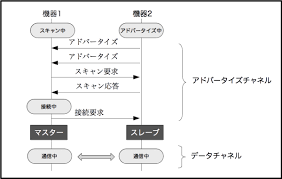
\includegraphics[width=10cm]{figures/ble_event.png}
    \caption{BLEの通信フロー}
    \label{fig:ble_event_flow}
    \end{center}
\end{figure}

\begin{table}[]
    \caption{LE packet structure}\label{fig:BLE_LE_PACKET_STRUCTURE}
    \centering
    \begin{tabular}{|c|c|c|c|}
    \hline
    \begin{tabular}[c]{@{}c@{}}Preamble\\ (1 octet)\end{tabular} & \begin{tabular}[c]{@{}c@{}}Access Address\\ (4 octets)\end{tabular} & \begin{tabular}[c]{@{}c@{}}PDU\\ (2 to 39 octets)\end{tabular} & \begin{tabular}[c]{@{}c@{}}CRC\\ (3 octets)\end{tabular} \\ \hline
    \end{tabular}
\end{table}

\begin{table}[]
    \caption{Advertising Channel PDU}\label{fig:BLE_ADV_CHANNEL_PDU}
    \centering
    \begin{tabular}{|c|c|c|}
    \hline
    \begin{tabular}[c]{@{}c@{}}Header\\ (2 octets)\end{tabular} & \begin{tabular}[c]{@{}c@{}}Advertiser's Address\\ (6 octets)\end{tabular} & \begin{tabular}[c]{@{}c@{}}Advertiser's Data\\ up to 31 octets\end{tabular} \\ \hline
    \end{tabular}
\end{table}